\documentclass{article}
\usepackage{amsmath}
\usepackage{amssymb}
\usepackage{graphicx}
\usepackage{float}
\usepackage{hyperref}
\usepackage{fancyvrb}
\usepackage{matlab-prettifier}
\setlength{\parindent}{0pt}
\graphicspath{{../images/}}

\title{CS663: Digital Image Processing - Homework 3}
\author{Harsh $\vert$ Pranav $\vert$ Swayam} 
\date{October 1, 2024}

\begin{document}

\maketitle
\section{Homework 3 - Question 4}

% Consider a \( 201 \times 201 \) image whose pixels are all black except for the central column (i.e., column index 101, beginning from 1 to 201) in which all pixels have the value 255. Derive the Fourier transform of this image analytically, and also plot the logarithm of its Fourier magnitude using \texttt{fft2} and \texttt{fftshift} in MATLAB. Use appropriate colorbars.

% \section*{Solution}

The Fourier transform of such an image can be computed as follows:

\[
F(u,v) = \frac{1}{201} \sum_{x=1}^{201} \sum_{y=1}^{201} \delta(x - 101) e^{-j 2\pi \left( \frac{ux}{201} + \frac{vy}{201} \right)}
\]

Since the image is zero everywhere except in the 101st column, we can simplify the summation by fixing \( x = 101 \):

\[
F(u,v) = \frac{1}{201} \sum_{y=1}^{201} 255 \cdot e^{-j 2\pi \left( \frac{101u}{201} + \frac{vy}{201} \right)}
\]

Factoring out constants, we get:

\[
F(u,v) = \frac{255}{201} e^{-j 2\pi \frac{101u}{201}} \sum_{y=1}^{201} e^{-j 2\pi \frac{vy}{201}}
\]

The summation is a geometric series, and it evaluates to:

\[
F(u,v) = \frac{255}{201} e^{-j 2\pi \frac{101u}{201}} \cdot \frac{1 - e^{-j 2\pi v}}{1 - e^{-j \frac{2\pi v}{201}}}
\]

This evaluates to:

\[
F(u,v) = \begin{cases}
K e^{-j 2\pi \frac{101u}{201}} \cdot 201, & v = 201n, \quad n \in \mathbb{Z}, \\
K e^{-j 2\pi \frac{101u}{201}} \cdot \frac{1 - e^{-j 2\pi v}}{1 - e^{-j \frac{2\pi v}{201}}}, & \text{otherwise}
\end{cases}
\]

where \( K \) is a constant.

This is zero when \( v \) is an integer not divisible by 201.

\section*{MATLAB Code}

The following MATLAB code computes the Fourier transform using \texttt{fft2}, shifts the zero frequency component to the center using \texttt{fftshift}, and plots the logarithm of the Fourier magnitude:

\begin{verbatim}
% MATLAB code to compute the Fourier transform
I = zeros(201, 201); % Create a 201x201 black image
I(:, 101) = 255; % Set the central column to 255

% Compute the 2D Fourier transform and shift zero-frequency to center
F = fft2(I);
F_shifted = fftshift(F);

% Compute the logarithm of the magnitude
log_magnitude = log(abs(F_shifted) + 1);

% Plot the result
figure;
imagesc(log_magnitude);
colorbar;
title('Logarithm of Fourier Magnitude');
\end{verbatim}

\section*{Output Image}

The output image is shown in Figure \ref{fig:q4}.
\begin{figure}[H]
    \centering
    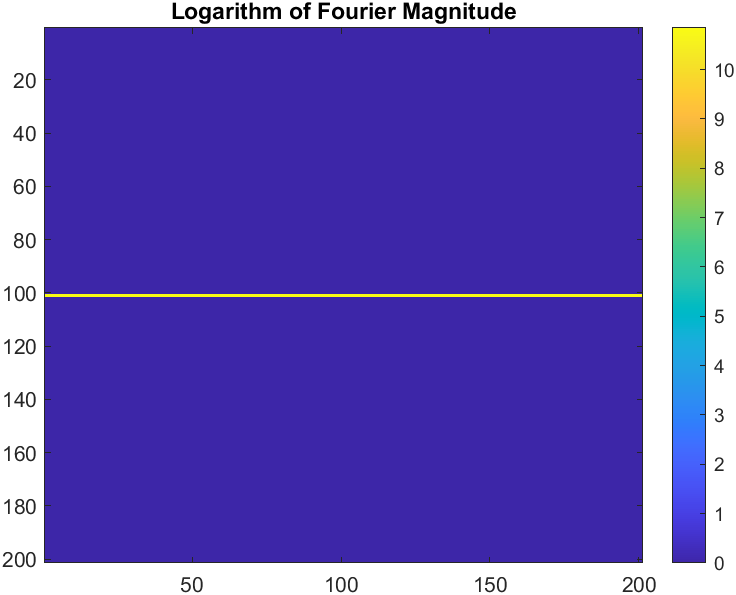
\includegraphics[width=0.5\textwidth]{fourier_output.png}
    \caption{Logarithm of Fourier Magnitude}
    \label{fig:q4}
\end{figure}

\section*{Conclusion}

The Fourier transform of the given image has been derived analytically and computed using MATLAB. The image contains a strong response along the vertical frequency components due to the constant value in the central column of the image.

\end{document}